% Do not change the options here
\documentclass[bsc,frontabs,parskip,deptreport]{infthesis}

\usepackage{graphicx}
\usepackage[%  
    colorlinks=true,
    pdfborder={0 0 0},
    linkcolor=red,
    citecolor=blue
]{hyperref}


\begin{document}
\begin{preliminary}
\title{A Zoom filter for applause and laughter}

\author{Lasse Wolter}

% to choose your course
% please un-comment just one of the following
%\course{Artificial Intelligence}
\course{Artificial Intelligence and Computer Science}
%\course{Artificial Intelligence and Mathematics}
%\course{Artificial Intelligence and Software Engineering}
%\course{Artificial Intelligence with Management}
%\course{Cognitive Science}
%\course{Computer Science}
%\course{Computer Science and Management Science}
%\course{Computer Science and Mathematics}
%\course{Computer Science and Physics}
%\course{Computer Science with Management}
%\course{Software Engineering}
%\course{Software Engineering with Management}

\project{4th Year Project Report}

\date{\today}

\abstract{

% This skeleton demonstrates how to use the \texttt{infthesis} style for
% undergraduate dissertations in the School of Informatics. It also emphasises the
% page limit, and that you must not deviate from the required style.
% The file \texttt{skeleton.tex} generates this document and can be used as a
% starting point for your thesis. The abstract should summarise your report and
% fit in the space on the first page.
}

\maketitle

\section*{Acknowledgements}


\tableofcontents
\end{preliminary}


% The preliminary material of your report should contain:
% \begin{itemize}
% \item
% The title page.
% \item
% An abstract page.
% \item
% Optionally an acknowledgements page.
% \item
% The table of contents.
% \end{itemize}

\chapter{Introduction}

\chapter{Background}
Automatic applause and laughter detection isn't a new idea. Nevertheless, the research in these two areas is usually done separately. There are a few papers which cover both, laughter and applause detection, one of the most popular ones being from Cai et. al \cite{cai2003highlight} who used sound effect detection - which included laughter and applause - for video summarisation and highlight extraction.
Apart from this and a few other papers most research only covers one of the two domains, either applause or laughter. Thus, we split the review of existing research into the following sections:
\begin{enumerate}
  \item Laughter Detection
  \item Applause Detection
  \item Brief introduction into audio processing
\end{enumerate}


\section{Laughter Detection}
The investigation of the acoustic features of laughter reaches back three decades \cite{bickley1992acoustic}. The first attempts of laughter detection were done in the early 2000s \cite{kennedy2004laughter, truong2005automatic}.
Corpora used in these papers include the ICSI Meeting Recorder corpus \cite{morgan2001meeting}, the CMU, LDC, NIST recordings as well as the Dutch CGN corpus. 
Kennedy and Ellis \cite{kennedy2004laughter} got the best results using Mel Frequency Cepstral Coefficients (MFCCs) as features and a Support Vector Machine (SVM) for decision making. 
MFCCs are one of the most widely used features in speech recognition and make use of the spectral representation of an audio wave (Section \ref{theory}).

In contrast to Kennedy and Ellis \cite{kennedy2004laughter}, Truong and Van Leeuwen \cite{truong2005automatic} used Perceptual Linear Prediction (PLP) features with Gaussian Mixture Models (GMM) for classification. 
We further note that not only the features and predictors differ, also the motivation and definition of laughter events differ. 
While Kennedy and Ellis define laughter events as 'points in the meeting where more than one person laughs', Truong and Van Leeuwen already considered one person laughing as laughter event.
Kennedy and Ellis didn't specify a particular motivation whereas Truong and Van Leeuwen's long-term goal was the investigation of 'paralinguistic events' - laughter being one of them - to classify the speaker's emotional state.   

Both of these early papers on laughter recognition worked with presegmented laughter samples where predictions only classified a segment as laughter or non-laughter. The determination of segment boundaries of laughter events - which is key for our project - wasn't considered. 

Truong and Leeuwen \cite{truong2007automatic} continued their research and stated that spectral features alone (such as PLP and MFCCs) can be used to discriminate between laughter and speech but a significant improvement can be achieved when using prosodic features - features relating the rhythm and intonation.

Knox and Mirghafori \cite{knox2006automatic} were the first to do laughter recognition without presegmented data.
They also worked with the ICSI Meeting corpus \cite{morgan2001meeting} and used a single layer neural network for classification.
Instead of classifying presegmented snippets they classified each 10ms frame using a window of 75 frames around the target frame - 37 before and after the frame (\ref{fig:know_window}).
That way an accurate prediction of laughter boundaries of up to 10ms was possible. 
Knox and Mirghafori obtained the best results by combining the output of three NN-systems which used delta MFCCs (derivatives of MFCCs), AC PEAK and F0 as features, respectively. While MFCCs are spectral features, AC PEAK and F0 are prosodic featuers relating to the pitch and energy of the sound.
The best system achieved an Equal Error Rate (EER) of 7.91\%.
They observed that of all tested features MFCCs have the most discriminative power which aligns with prior research by Kennedy and Ellis \cite{kennedy2004laughter}.

\begin{figure}[htp]
    \centering
    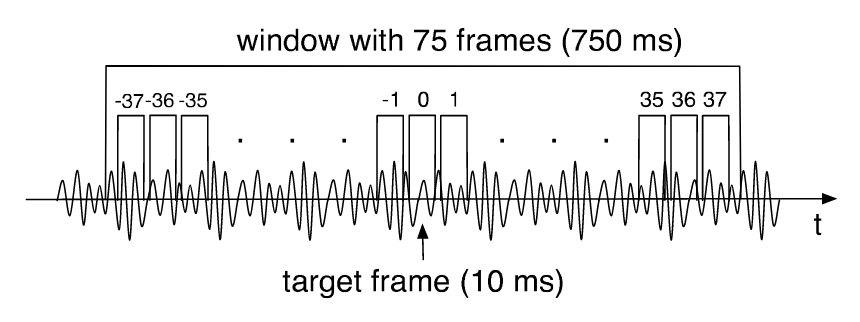
\includegraphics[width=10cm]{imgs/Knox_window.png}
    \caption{Frame window used by Know and Mirghafori}
    \label{fig:know_window}
\end{figure}

A survey from 2016 \cite{cosentino2016quantitative} investigates research on laughter and laughter detection in different fields up to that time.
This survey covers different detection methods, using visual, acoustic and sensory data.
For our specific problem we'd like to focus on acoustic data for two reasons.
On the one hand, people might have privacy concerns if their visual input is used for classification.
On the other hand, in video meetings and conferences people often turn off their video input.
Consentino et al. \cite{cosentino2016quantitative} also mention the privacy implications of video input and raise the same concern for audio input.
Thus, they suggest the use of individual wearable sensors to address these concerns.
For our project this approach isn't feasible and further, wearable devices might be quite intrusive.
In our system people can opt-out of using the laughter-detection feature at any time.
That way people stay in control of their own privacy.

For laughter detection using solely acoustic data, Consentino et al. \cite{cosentino2016quantitative} find that best performance in prior research was obtained using MFCCs and PLPs as features and combining the resulting classifier with ones that also use prosodic features.
This aligns with findings from prior research \cite{truong2007automatic, knox2006automatic}.

More recent research by Gillick et al. \cite{gillick2021robust} finds that features learned from spectrograms using deep convolutional networks outperform previous approaches based on MFCCs.
Their hypothesis was that models using MFCCs are more prone to pick up surface level characteristics of sound and thus, will be more sensitive to variations like background noise.
Gillick et al. expected that features learned using a CNN are more representative of the actual laughter and thus, more robust to different environments. 
Their results suggest that their hypothesis might be correct.
The results definitely show that the features learned by a CNN architecture (with or without data augmentation) outperform the conventional approach using MFCCs. 


\section{Applause}
The following review is less exhaustive compared to the review on laughter detection.
This is due to the fact that we decided to focus on laughter detection for now and possibly add applause detection afterwards.
More information on this decision can be found (TODO: Link to corresponding section).

As mentioned at the beginning of this chapter, in 2003 Cai et al. \cite{cai2003highlight} worked on the detection of sound events, including but not limited to applause.
They used perceptual features and MFFCs as features, Hidden Markov Models (HMM) and Gaussian Mixture models (GMM) to model sound and log likelihood for decision making.
Cai et al. evaluated their system on a testing set consisting of 2 hours of video material from different programs.
For applause specifically they achieved a precision of 87.37\% and a recall of 92.00\%.

In contrast, Uhle \cite{uhle2011applause} used MFCCs and low-level descriptors (LLD) to represent sound and passed these features to an MLP or an SVM for classification.
The difference between MLP and SVM classifier were rather small which is why both are mentioned here.
Uhle worked with a relatively small data set consisting of 210 snippets of 9-30s length. This equates to a total length between 31.5 min and 105 min.
On a rather small test (10\% of the whole data set) Uhle achieved an accuracy of 95\% with a precision 96.51\% and recall of 97.65\%.

A less complex approach for applause detection was presented by Li et al. \cite{li2009characteristics}.
They used a 4-layer decision tree to classify a given sound input as applause or not-applause.
Testing their model on 50 hours of meeting speech containing 500 applause segments ranging from 0.8 to 0.36s they were able to retrieve 491 of the 500 applause segments while incorrectly retrieving 38 non-applause segments.
This equates to a recall of 98.2\% and a precision of 92.82\%. Li et al. also compared their less complex model to the HMM model proposed by Cai et al.\cite{cai2003highlight} and outperformed it while using less computational time.

Manoj et. al \cite{manoj2011novel} proposed another approach based on decision trees and also compared it to a more complex model similar to the one proposed by Cai et al. \cite{cai2003highlight} - using only GMMs, no HMMs.
Even though the decision tree stages are different to Li et al. \cite{li2009characteristics} the findings align. The decision tree outperforms the more complex method using MFCCs and GMMs.  

\section{Brief introduction into audio processing} \label{theory}
Possible topics one could talk about
\begin{itemize}
    \item Preprossing: 
    \begin{itemize}
        \item Conversion from audio wave to spectrogram 
        \item Data Augmentation
    \end{itemize}
    \item Some details on MFCCs 
\end{itemize}


\bibliographystyle{plain}
\bibliography{mybibfile}

%% You can include appendices like this:
% \appendix
%
% \chapter{First appendix}
%
% \section{First section}
%
% Markers do not have to consider appendices. Make sure that your contributions
% are made clear in the main body of the dissertation (within the page limit).

\end{document}
